%
% main.tex -- Paper zum Thema arctan
%
% (c) 2020 Hochschule Rapperswil
%
\chapter{Kettenbrüche und Padé-Approximation\label{chapter:arctan}}
\lhead{Kettenbrüche und Padé-Approximation}
\rhead{}
\begin{refsection}
\chapterauthor{Andreas Müller}

{\parindent0pt
Kettenbrüche} versprechen eine bestmögliche Approximation einer Zahl durch
rationale Zahlen, die Padé-Approximation verspricht eine bestmögliche
Approximation einer Potenzreihe durch eine gebrochen rationale Funktion.
Besteht ein Zusammenhang?

In Kapitel~\ref{chapter:kettenbruch} wurde ohne Beweis eine Approximation der 
Taylor-Reihe der Arkustangens-Funktion
\begin{equation}
\arctan x
=
x-\frac{x^3}{3}+\frac{x^5}{5}-\frac{x^7}{7}+\frac{x^9}{9}-\frac{x^{11}}{11}
+\dots
\label{arctan:arctan}
\end{equation}
als Kettenbruch präsentiert.
Doch genau genommen ist das gar kein Kettenbruch in dem Sinne, wie er
im Rest von Kapitel~\ref{chapter:kettenbruch} betrachtet wurde, denn
bestimmt man die Approximationsbrüche, entstehen nicht Brüche von ganzen
Zahlen sondern eine gebrochen rationale Funktion.
In diesem Kapitel soll gezeigt werden, dass der Kettenbruch eigentlich
nur eine Schreibweise ist, mit der verschiedene Padé-Approximanten von
$\arctan x$ effizient berechnet werden können.

\section{Kettenbrüche und Matrizen
\label{arctan:section:matrizen}}
\rhead{Kettenbrüche und Matrizen}
Wir verwenden wieder die schon in Kapitel \ref{chapter:kettenbruch}
eingeführte Notation
\[
\frac{p_n}{q_n}
=
a_0 +
\cfrac{b_1}{
a_1+\cfrac{b_2}{
a_2+\cfrac{b_3}{
\dots+\cfrac{\dots}{\dots+\cfrac{b_{n-1}}{a_{n-1}+\cfrac{b_n}{a_n}}}}}}.
\]
Für einen Kettenbruch hatten verlangt, dass alle Zahlen $a_k$ und $b_k$ 
wie auch die Zähler $p_n$ und Nenner $q_n$ der Näherungsbrüche
ganze Zahlen sind.
Für die Approximation der Funktion $\arctan x$ müssen wir
diese Voraussetzung etwas aufweichen.
Wir verlangen nur noch, dass alle diese Ausdrücke Polynome in $x$ sind.

Wir brauchen eine Methode zur Berechnung der Approximationszähler und -nenner.
Dazu berechnen wir, wie sich ein Bruch ändert, wenn ein zusätzlicher
Bruchterm $\frac{p}{q}$ im Nenner hinzugefügt wird:
\begin{equation}
\frac{\tilde{p}}{\tilde{q}}
=
\cfrac{b}{a+\cfrac{p}{q}}
=
\frac{bq}{ab+p}.
\label{arctan:neuerbruch}
\end{equation}
Schreibt man die Brüche als Spaltenvektoren mit Zähler und Nenner als
Komponenten, dann kann man die Operation~\eqref{arctan:neuerbruch}
in Matrixform als
\[
\begin{pmatrix}
\tilde{p}\\\tilde{q}
\end{pmatrix}
=
\begin{pmatrix}
bq\\
aq+p
\end{pmatrix}
=
\begin{pmatrix}
0&b\\
1&a
\end{pmatrix}
\begin{pmatrix}
p\\
q
\end{pmatrix}
\]
schreiben.
Durch Iteration dieser Idee kann man daher den Näherungsbruch $p_n/q_n$
ebenfalls in Matrixform als
\[
\begin{pmatrix}
p_n\\q_n
\end{pmatrix}
=
\begin{pmatrix} 0&b_1\\1&a_1\end{pmatrix}
\begin{pmatrix} 0&b_2\\1&a_2\end{pmatrix}
\begin{pmatrix} 0&b_3\\1&a_3\end{pmatrix}
\dots
\begin{pmatrix} 0&b_{n-1}\\1&a_{n-1}\end{pmatrix}
\begin{pmatrix} b_n\\a_n\end{pmatrix}
\]
schreiben.
Will man den letzten Bruch $b_n/a_n$ in der Kettenbruchentwicklung
weglassen, also den Kettenbruch verkürzen, dann ist das gleichbedeutend
damit, $b_n=0$ und $a_n=1$ zu setzen.
Damit erhält man aber die Approximation $p_{n-1}/q_{n-1}$.
Kombiniert man beide Approximationen in eine Matrix, erhält man
\begin{equation}
\begin{pmatrix}
p_{n-1}&p_n\\
q_{n-1}&q_n
\end{pmatrix}
=
\begin{pmatrix} 0&b_1\\1&a_1\end{pmatrix}
\begin{pmatrix} 0&b_2\\1&a_2\end{pmatrix}
\begin{pmatrix} 0&b_3\\1&a_3\end{pmatrix}
\dots
\begin{pmatrix} 0&b_{n-1}\\1&a_{n-1}\end{pmatrix}
\begin{pmatrix} 0&b_n\\1&a_n\end{pmatrix}.
\label{arctan:produkt}
\end{equation}

Das Produkt~\eqref{arctan:produkt} wurde oben zunächst von rechts nach links
abgeleitet, es wurde der ``letzte'' Ausdruck in Matrixform gebracht und
dann nach links fortschreitend der ganze Kettenbruch aufgebaut.
Die Matrixmultiplikation ist jedoch assoziativ, so dass man ausgerüstet
mit Formel~\eqref{arctan:produkt} die Quotienten $p_n/q_n$ jetzt auch von
links nach rechts berechnen kann.

\section{Padé-Approximation von $\arctan x$
\label{arctan:section:kettenbruch}}
\rhead{Padé-Approximation von $\arctan x$}
Wir versuchen jetzt zu verstehen, wie man die Taylor-Reihe~\ref{arctan:arctan}
als Kettenbruch deuten kann.
Nach dem Prinzip der Padé-Approximation suchen wir einen Bruch $p_n/q_n$,
der mit der Taylor-Reihe bis zu einem gewissen Grad $k$ übereinstimmt.
Wir verlangen daher, dass $p_n$ und $q_n$ Polynome sind, für die gilt
\[
\frac{p_n(x)}{q_n(x)} = \arctan x + O(x^{k+1}).
\]
Wir werden später sehen, dass wir $k=2n+1$ verlangen können, was zum
Beispiel bedeutet, dass $p_2(x)/q_2(x)$ mit der Reihe~\ref{arctan:arctan}
bis und mit Termen fünfter Ordnung übereinstimmt.
Wie bei der Herleitung der Padé-Approximation in Kapitel~\ref{chapter:pade}
multiplizieren wir mit dem Nenner und erhalten die Bedingung
\begin{equation}
p_n(x) - q_n(x)\arctan x = O(x^{k+1}).
\label{arctan:bedingung}
\end{equation}
Auch diese Bedingung lässt sich in Vektorform fassen:
\begin{align}
\begin{pmatrix}
1&-\arctan x
\end{pmatrix}
\begin{pmatrix} 
p_n(x)\\q_n(x)
\end{pmatrix}
&=
O(x^{k+1})
\notag
\\
\text{oder}\qquad
\begin{pmatrix}
1&-\arctan x
\end{pmatrix}
\begin{pmatrix}
p_{n-1}(x)&p_n(x)\\
q_{n-1}(x)&q_n(x)
\end{pmatrix}
&=
\begin{pmatrix}
O(x^{k})&O(x^{k+1}).
\end{pmatrix}
\label{arctan:bedingungmatrix}
\end{align}
Die Rekursionsfolge startet mit der Matrix
\begin{align*}
\begin{pmatrix}
1&-\arctan x
\end{pmatrix}
\begin{pmatrix}
p_0(x)&p_1(x)\\
q_0(x)&q_1(x)
\end{pmatrix}
&=
\begin{pmatrix}
1&-\arctan x
\end{pmatrix}
\begin{pmatrix}
0&p_1(x)\\
1&q_1(x)
\end{pmatrix}
\\
&=
\begin{pmatrix}
0
&
p_1(x) - q_1(x)
\biggl(\displaystyle x-\frac{x^3}{3}+\frac{x^5}{5}-\frac{x^7}{7}+\dots\biggr)
\end{pmatrix}.
\end{align*}
Damit auf der rechten Seite in der zweiten Komponente die Terme erster Ordnung
wegfallen, müssen $p_1$ und $q_1$ als Polynome möglichst niedrigen Grades
so gewählt werden, dass
\[
p_1(x)-xq_1(x) = O(x^2),
\]
dies kann zum Beispiel $q_1(x)=1$ und $p_1(x)=x$ geschehen.
Damit ist
\[
\begin{pmatrix}
p_0(x)&p_1(x)\\
q_0(x)&q_1(x)
\end{pmatrix}
=
\begin{pmatrix}
0&x\\
1&1
\end{pmatrix}
\]
der Start der Rekursion.

\subsection{Approximation bis zur Ordnung 3}
Die Bedingung \eqref{arctan:bedingungmatrix} kann jetzt dazu verwendet werden,
auch die weiteren $a_k$ und $b_k$ zu bestimmen.
Für $a_1$ und $b_1$ rechnen wir dazu zunächst das Produkt
\[
\begin{pmatrix}
p_0(x)&p_1(x)\\
q_0(x)&q_1(x)
\end{pmatrix}
\begin{pmatrix}
0&b_1\\
1&a_1
\end{pmatrix}
=
\begin{pmatrix}
0&x\\
1&1
\end{pmatrix}
\begin{pmatrix}
0&b_1\\
1&a_1
\end{pmatrix}
=
\begin{pmatrix}
x&a_1x\\
1&a_1+b_1
\end{pmatrix}
\]
aus. 
Multiplikation von links mit dem Zeilenvektor ergibt
\[
\begin{pmatrix}
1&-\arctan x
\end{pmatrix}
\begin{pmatrix}
x&a_1x\\
1&a_1+b_1
\end{pmatrix}
=
\begin{pmatrix}
O(x^3) & a_1x - (a_1+b_1)\biggl(\displaystyle x-\frac{x^3}3+O(x^5)\biggr)
\end{pmatrix}.
\]
Die Polynome $a_1$ und $b_1$ müssen so gewählt werden, dass keine Terme
dritter Ordnung mehr stehen bleiben.
Dies ist natürlich nicht eindeutig möglich sondern nur bis auf ein
Vielfaches.
Den Term erster Ordnung kann man mit konstantem $a_1$ zum verschwinden
bringen, dann muss aber $b_1$ mindestens den Grad $2$ haben.
Es muss also
\[
a_1x-(a_1+cx^2)\biggl(x-\frac{x^3}3+O(x^5)\biggr)
=
a_1\frac{x^3}{3}-cx^3 + O(x^5)
\]
sein.
Dies lässt sich zum Beispiel mit $a_1=3$ und $c=1$ erreichen.
Der Näherungsbruch ist dann
\[
\begin{pmatrix}
p_1(x)&p_2(x)\\
q_1(x)&q_2(x)
\end{pmatrix}
=
\begin{pmatrix}
x&3x\\
1&x^2+3
\end{pmatrix}
\qquad\Rightarrow\qquad
\frac{p_2(x)}{q_2(x)} = \frac{3x}{3+x^2}.
\]

\subsection{Approximation bis zur Ordnung 5}
Wir führen auch noch den Schritt $k=2$ durch, bei dem die Terme fünfter
Ordnung wegfallen sollten.
Das Matrizenprodukt ist
\[
\begin{pmatrix}
x&3x\\
1&x^2+3
\end{pmatrix}
\begin{pmatrix}
0&b_2\\
1&a_2
\end{pmatrix}
=
\begin{pmatrix}
3x    & b_2x + 3xa_2 \\
x^2+3 & b_2 + a_2(x^2+3)
\end{pmatrix}.
\]
Nach Linksmultiplikation mit dem Zeilenvektor ergibt sich wieder
\begin{align*}
b_2p_1(x) &+ a_2p_2(x) - (b_2q_1(x)+a_2q_2(x))
\arctan x
\\
&=
b_2(p_1(x)-q_1(x) \arctan x)
+ a_2(p_2(x) - q_2(x)\arctan x)
=
O(x^7).
\end{align*}
Im ersten Term wissen wir, dass wir, dass bereits die Terme der
Ordnung $\le 1$ wegfallen.
In der zweiten Klammer fallen die Terme bis zur dritten Ordnung weg.
Es folgt daher wieder, dass man für $b_2$ einen Term zweiten Grades
der Form $cx^2$ wählen muss und folglich für $a_2$ eine Konstante.
Setzt man alles ein, erhält man
\begin{align*}
cx^2\biggl(x- x+\frac{x^3}3-\frac{x^5}5+O(x^7)\biggr)
&+
a_2\biggl(3x -(x^2+3)\biggl(x-\frac{x^3}3+\frac{x^5}5+O(x^7)\biggr)\biggr)
\\
&=
c\frac{x^5}{3}
+O(x^7)
+a_2
\biggl(\frac{x^5}{3}-\frac{3}{5}x^5+O(x^7)\biggr)
\\
&=x^5\biggl(\frac{c}3-a_2\frac{4}{15}\biggr) + O(x^7),
\end{align*}
woraus als mögliche Lösung
\[
b_2=4x^2,\qquad
a_2=5
\]
folgt.
Der zugehörige Näherungsbruch ist
\[
\arctan x
\approx
\frac{p_3(x)}{q_3(x)}
=
\frac{xb_2+3xa_2}{b_2+a_2(x^2+3)}
=
\frac{4x^3+15x}{9x^2+15}.
\]

Es lässt sich zum Beispiel mit einem Computer-Algebra-Programm wie
Maxima verifizieren, dass die Matrizen
\begin{equation}
\begin{pmatrix}
0&b_n\\
1&a_n
\end{pmatrix}
=
\begin{pmatrix}
0&n^2x^2\\
1&2n+1
\end{pmatrix}
\qquad\text{also}\qquad
b_n=n^2x^2\qquad\text{und}\qquad a_n=2n+1
\label{arctan:increment}
\end{equation}
tatsächlich dafür sorgen, dass die Kettenbruchentwicklung 
immer eine Approximation bis zur Ordnung $2n+1$ ist.
Damit erhalten wir den Kettenbruch
\[
\arctan x
=
\cfrac{x}{
1+\cfrac{x^2}{
3+\cfrac{4x^2}{
5+\cfrac{9x^2}{
7+\cfrac{16x^2}{
9+\dots
}}}}},
\]
den wir bereits in Kapitel~\ref{chapter:kettenbruch} gefunden haben.

Mit Computerhilfe kann man jetzt die folgenden Näherungsbrüche ausrechnen:
\begin{align*}
\frac{p_1(x)}{q_1(x)} &= \frac{x}{1},
\\
\frac{p_2(x)}{q_2(x)} &= \frac{3x}{x^2+3},
\\
\frac{p_3(x)}{q_3(x)} &= \frac{4x^3+15x}{9x^2+15},
\\
\frac{p_4(x)}{q_4(x)} &= \frac{55x^3+105x}{9x^4+90x^2+105},
\\
\frac{p_5(x)}{q_5(x)} &= \frac{6x^5+735x^3+945x}{225x^4+1050x^2+945}.
\end{align*}
Ihre Graphen sind in Abbildung~\ref{arctan:figure:approx} dargestellt.
\begin{figure}
\centering
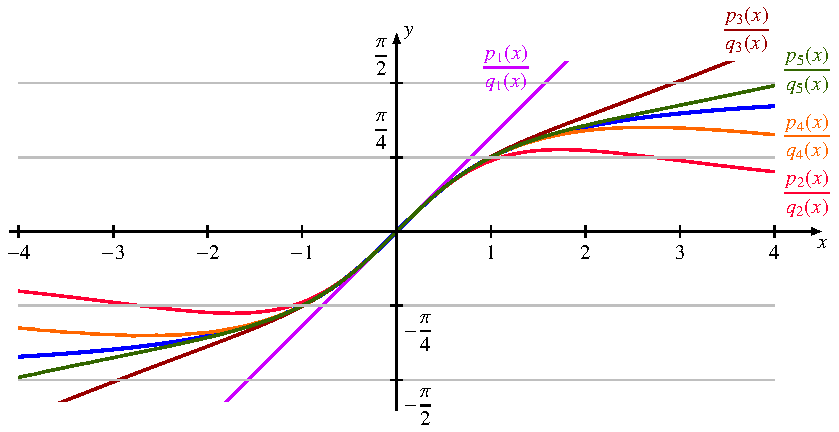
\includegraphics[width=\hsize]{papers/arctan/approx.pdf}
\caption{Graphen der Näherungsbrüche $p_n/q_n$ für die Funktion $\arctan x$
(blau)
für $n=1,\dots,5$.
Die Näherungsbrüche approximieren $\arctan x$ abwechselnd von oben und unten.
\label{arctan:figure:approx}}
\end{figure}

\subsection{Der Grad von Zähler und Nenner}
Wir ermitteln noch die Grade der Polynome $p_n$ und $q_n$.
Für den Grad $\deg p(x)$ eines Polynoms gelten die Rechenregeln
\begin{align*}
\deg 0&= -\infty,
\\
\det x^k&= k,
\\
\deg p(x) q(x) & = \deg p(x) + \deg q(x),
\\
\deg (p(x)+q(x)) &\le \max (\deg p(x),\deg q(x)).
\end{align*}
Damit lässt sich die Veränderung der Grade der Matrixeinträge bei
Matrizenprodukten nachvollziehen, wir nenne dies die {\em Grad-Multiplikation}.
Schreiben wir eckige Klammern für eine Matrix aus Graden, denn gelten
dafür die Rechenregeln
\[
\begin{bmatrix}
a_{11}&a_{12}\\
a_{21}&a_{22}
\end{bmatrix}
\begin{bmatrix}
b_{11}&b_{12}\\
b_{21}&b_{22}
\end{bmatrix}
=
\begin{bmatrix}
\max (a_{11} + b_{11}, a_{12}+b_{21})&\max (a_{11} + b_{12}, a_{12}+b_{22})\\
\max (a_{21} + b_{11}, a_{22}+b_{21})&\max (a_{21} + b_{12}, a_{22}+b_{22})
\end{bmatrix},
\]
die man aus der Definition des Matrizenproduktes erhält, indem man Produkte
durch Summen und Summen durch $\max(\;,\;)$ ersetzt.

Für den Speziallfall der Matrix \eqref{arctan:increment} gilt
\[
\deg
\begin{pmatrix}
0&n^2x^2\\
1&2n+1
\end{pmatrix}
=
\begin{bmatrix}
-\infty & 2\\
   0    & 0
\end{bmatrix}.
\]
Wir berechnen jetzt die Gradmatrizen für $p_n$ und $q_n$.
Zu Beginn gilt
\begin{align*}
\deg
\begin{pmatrix}
p_1(x)&p_2(x)\\
q_1(x)&q_2(x)
\end{pmatrix}
&=
\begin{bmatrix}
1&1\\
0&2
\end{bmatrix}.
\end{align*}
Für die späteren Näherungsbrüche berechnen wir gleich allgemeiner
\begin{align*}
\begin{bmatrix}
k&k\\
k-1&k+1
\end{bmatrix}
\begin{bmatrix}
-\infty & 2\\
   0    & 0
\end{bmatrix}
&=
\begin{bmatrix}
k&k+2\\
k+1&k+1
\end{bmatrix}
\\
\begin{bmatrix}
k&k+2\\
k+1&k+1
\end{bmatrix}
\begin{bmatrix}
-\infty & 2\\
   0    & 0
\end{bmatrix}
&=
\begin{bmatrix}
k+2&k+2\\
k+1&k+3
\end{bmatrix}.
\end{align*}
Daraus lesen wir ab, dass sich die Grade von Zähler und Nenner wie in Tabelle
\ref{arctan:ordnungen} entwickeln.
\begin{table}
\centering
\begin{tabular}{>{$}l<{$}| >{$}c<{$} >{$}c<{$} >{$}c<{$} >{$}c<{$} >{$}c<{$} >{$}c<{$} >{$}c<{$}}
n          & 1& 2& 3& 4& 5& 6& 7\\
\hline
\deg p_n(x)& 1& 3& 3& 5& 5& 7& 7\\
\deg q_n(x)& 2& 2& 4& 4& 6& 6& 8\\
\hline
\text{Ordnung}& 3& 5& 7& 9&11&13&15\\
\end{tabular}
\caption{Grade von Zähler und Nenner-Polynomen des Kettenbruchs für $\arctan x$.
Die letzte Zeile enthält die Ordnung, bis zu der $p_{n}(x)-q_n(x)\arctan x$
verschwindet.
\label{arctan:ordnungen}}
\end{table}
In Kapitel~\ref{chapter:pade} wurde gezeigt, dass diese Ordnungen auch
die Padé-Approximanten charakterisieren.
Der Näherungsbruch $p_n/q_n$ ist also ein Padé-Approximant von $\arctan x$,
und zwar ist
\[
\frac{p_n(x)}{q_n(x)}
=
\begin{cases}
\;[n+1/n]&\qquad \text{$n$ gerade}\\
\;[n/n+1]&\qquad \text{$n$ ungerade.}
\end{cases}
\]


\printbibliography[heading=subbibliography]
\end{refsection}
